\documentclass{pnastwo}
\usepackage{cite}
\usepackage{color}
\usepackage{pgf}
%\usepackage{hyperref}
\newcommand{\jri}[1]{\textcolor{blue}{\emph{#1}} }

\begin{document}

\title{Demography and selection since maize domestication}
\author{Timothy M. Beissinger\affil{1}{Dept. of Plant Sciences, University of
    California, Davis, CA, USA}, Li Wang\affil{2}{Iowa State University, Ames, IA, USA}, Arun
  Durvasula\affil{1}{}, Kate Crosby\affil{1}{}, Matthew Hufford\affil{2}{}, \and Jeffrey
  Ross-Ibrarra\affil{1}{}\affil{3}{Genome Center and Center for population biology, University of
    California, Davis, CA, USA} }

\significancetext{This work is insignificant ;-)}

\maketitle

\begin{article}

\begin{abstract}
This is the abstract. It should probably be somewhere around 200 words.
\end{abstract}

\dropcap{D}omesticated plant species evolve in a unique fashion
compared to their wild relatives \textcolor{red}{(ref here)}. This
is a result of both the anthropomorphic nature of artificial selection on
domesticates \cite{purugganan2009} as well as the demographic characteristics of the domestication
bottleneck that they tend to have experienced
\cite{ross2007}. However, the
complex interplay between selective pressures and demographic limitations in
domesticated species is not well understood. Despite the fact that,
researchers have searched the genomes of several species for evidence
of positive selection during domestication
\textcolor{red}{(citations here)}, these types of studies tend to focus on
identifying or mapping particular genes or regions that play an
important role in phenotypic evolution. Our knowledge regarding the impacts of demography and
selection have on whole-genome patterns of genetic variability therefore remain limited.

\textcolor{red}{
This is the beginning of the article. For now, I will give a
bulleted list of the introduction:
\begin{enumerate}
\item Plant domestication
\item Maize
\item Maize domestication
\item Importance of demography
\item Background selection
\end{enumerate}
}



\section{Results}
\subsection{Patterns of variability differ between genic and
  nongenic regions of the genome}
Previous research of the maize domestication process has relied upon
observations drawn from genic DNA \textcolor{red}{(several references
  here)}. Our data were generated through whole genome sequencing,
which eliminated this constraint. Importantly, we observed substantial
differences in patterns of diversity between genic and non-genic regions
of the genome for both maize and teosinte. For maize, mean pairwise
diversity ($\pi$) within genes was significantly lower than at
positions at least 5kb away from genes (0.00668 within, 0.00691 away, p$<$2e-44). The same
pattern of significantly greater diversity outside of genes was observed in
teosinte, but to a larger extent. For teosinte we observed $\pi$
within genes to be 0.0088 and at least 5kb from genes it was 0.1153
(p$\approx$0). These obserrvations suggest that genes are not evolving
neutrally in maize or teosinte. Instead, some form of selection is likely
reducing diversity within genes. Additionally, these observations
suggest that demographic inference, which relies on the assumption of
neutrally evolving DNA, will be more accurate if it is based on
observations from non-genic genetic material.

\subsection{Hard sweeps do not shape maize (or teosinte) diversity}
A mutation that is immediately beneficial and positively selected leaves a classical hard
sweep signature in the genome, whereby genetic diversity surrounding
that mutation is reduced as the haplotype where the mutation first
arose increases in frequency to fixation. The prevalence of such hard
sweeps was evaluated by comparing diversity
surrounding non-synonymous and synonymous substitutions in maize and
teosinte since divergence from \emph{Tripsacum}, roughly \textcolor{red}{ZZZ} years before
present \textcolor{red}{(ref here)}. For both taxa, no difference in diversity
surrounding these classes of substitutions was identified (Figure
\ref{hardSweeps}). Additionally, diversity around maize substitutions
not seen in teosinte was investigated. These sites have the potential
to correspond to recent maize sweeps, occuring after the split from
teosinte. Again, no difference was observed between diversity around
synonymous and nonsynonymous substitutions
\textcolor{red}{(Supplemental figure here)}. Together, these
observations suggest that hard sweeps are not a primary form of
selection for either maize or teosinte.

\begin{figure}[b]
%\vspace*{.05in}
\centering
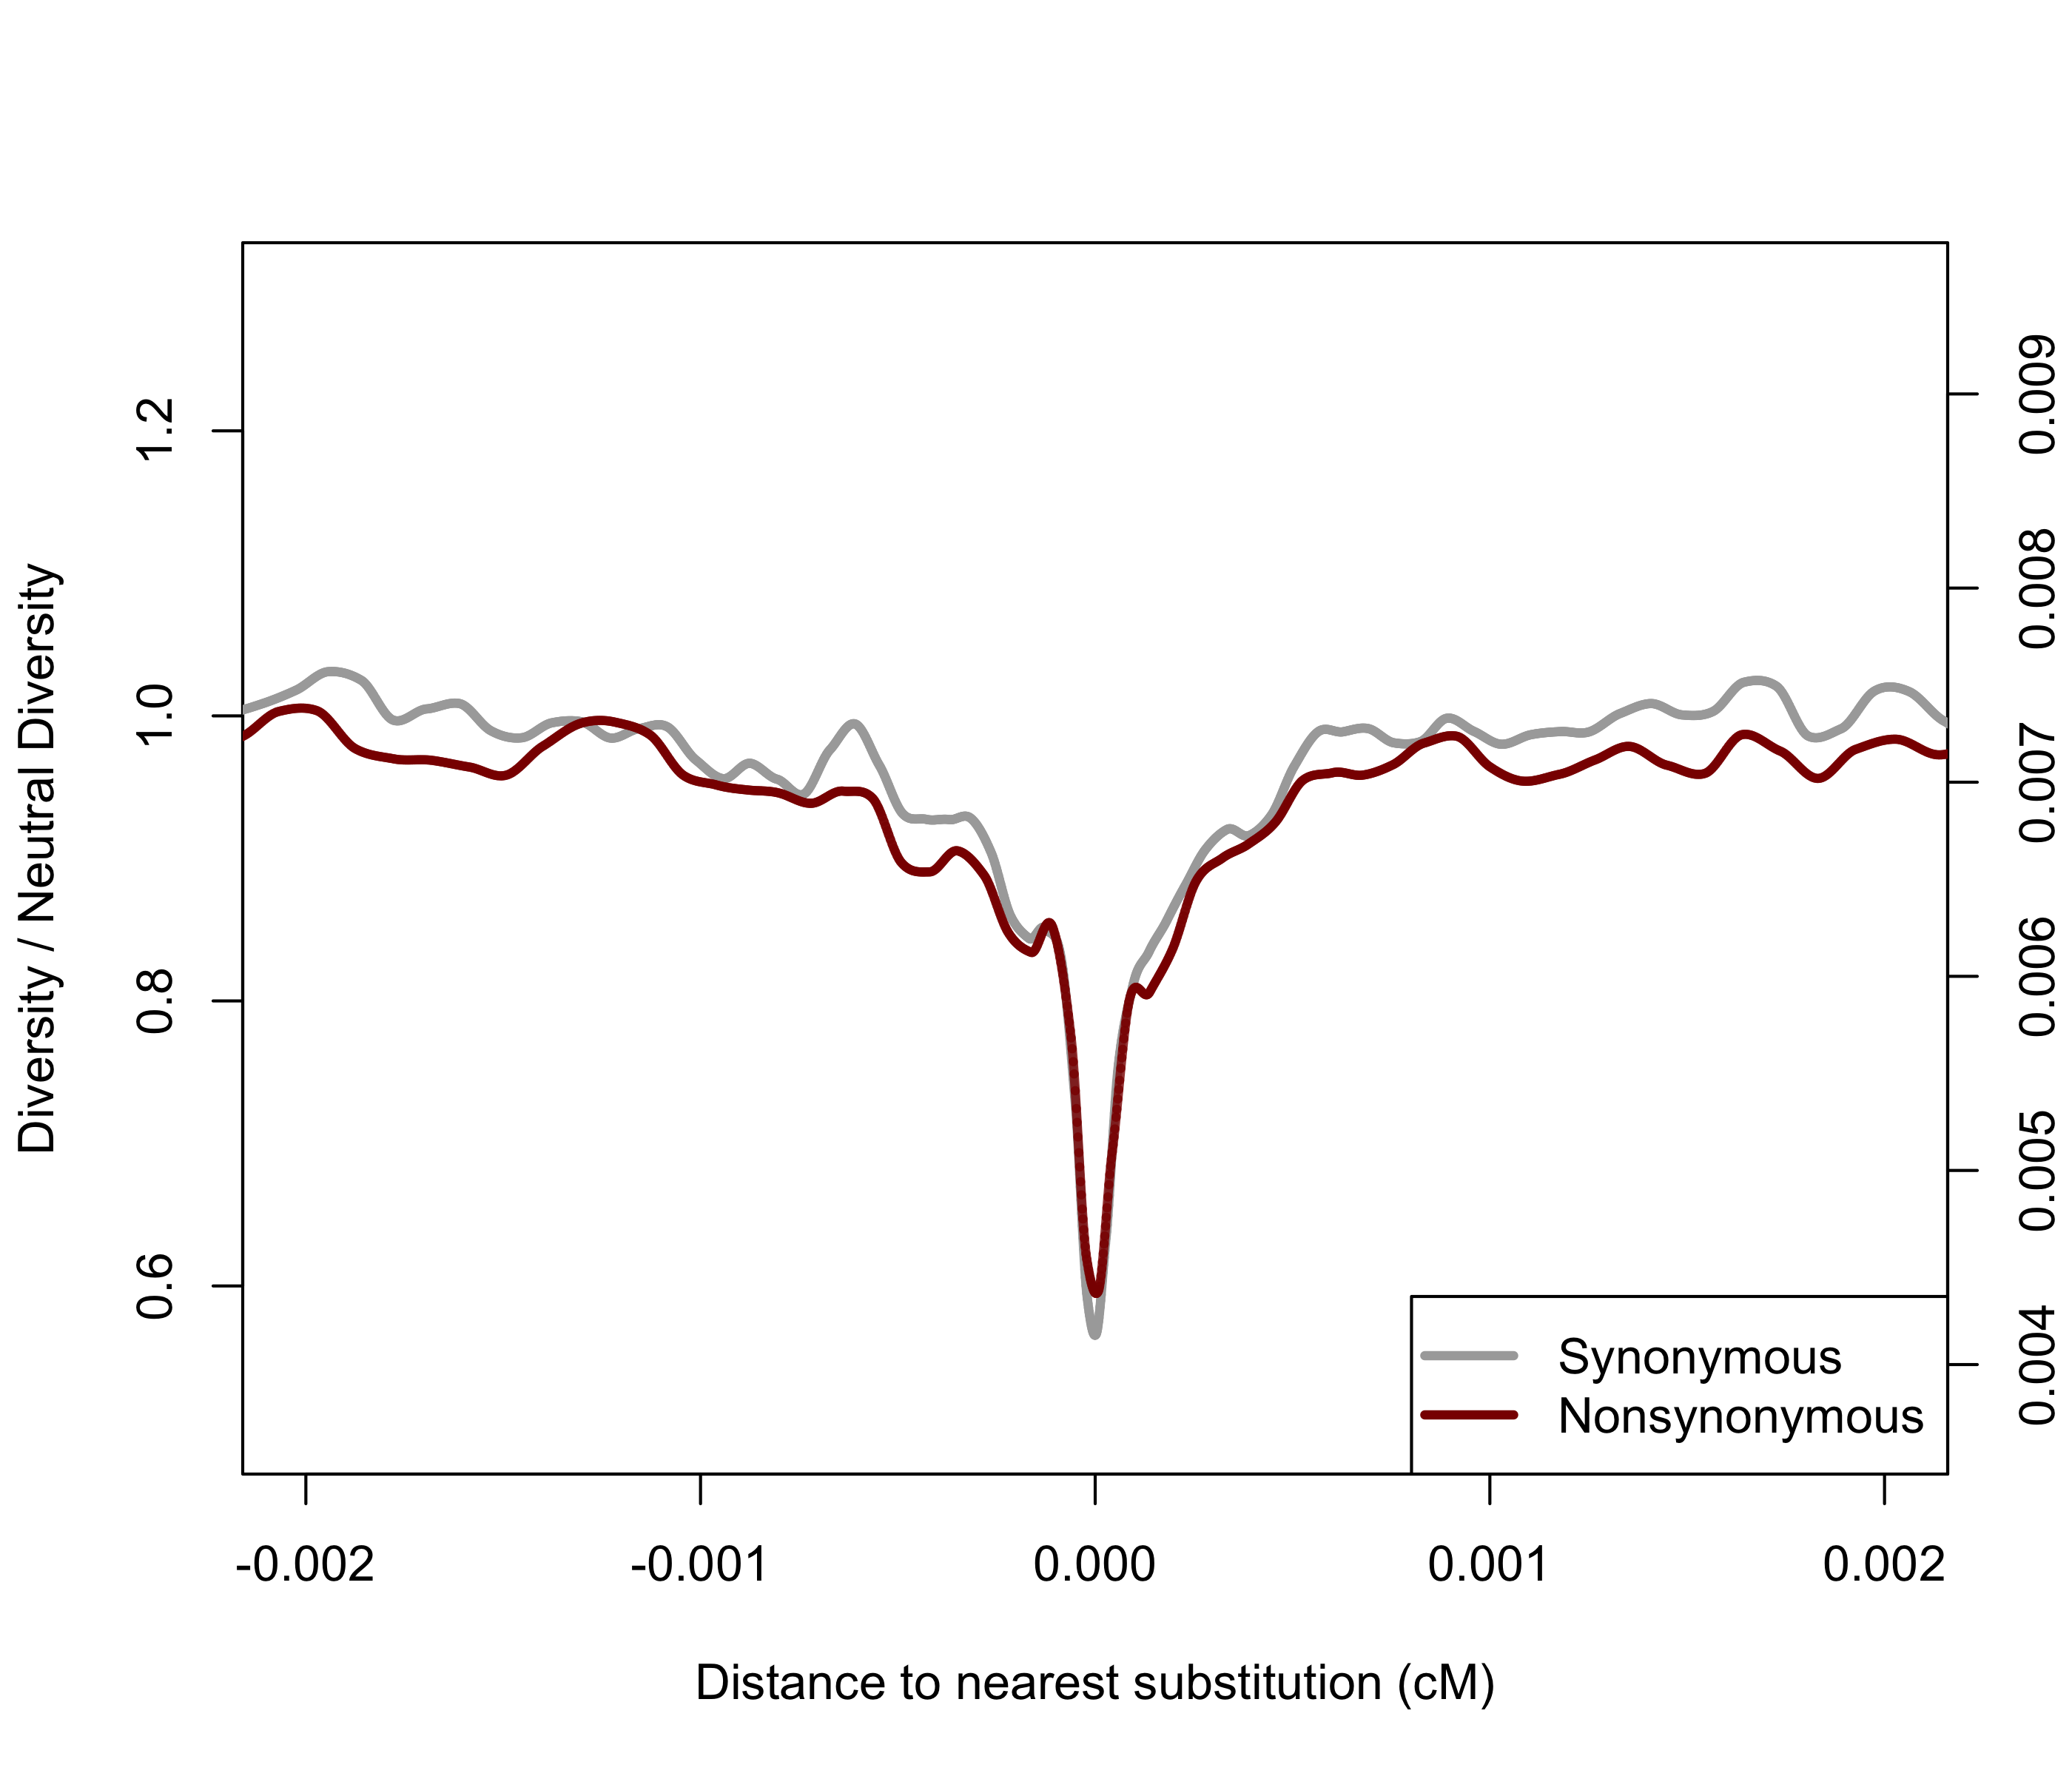
\includegraphics[width=.5\textwidth]{FigsAndFiles/plotDiversity_TvM_Folded2_unNeutralized}
\caption{Pairwise diversity surrounding synonymous and nonsynonymous
  substitutions in maize. \jri{needs larger legend/axis labels. x axis needs to say cM}}
\label{hardSweeps}
\end{figure}


\subsection{Patterns of purifying and background selection are
  influenced by demographic history}
Purifying selection refers to the situation where deleterious
mutations arising in a population are continuously selected against. When this
form of selection is operating, it can serve to reduce genetic
variability at linked neutral sites, a phenomenon called
background selection \cite{charlesworth1993}. Purifying and background selection lead
to lower diversity within genes and other functional sites relative
to neutral regions \textcolor{red}{(ref here)}. We investigated purifying
selection in maize and teosinte by evaluating the average magnitude of reduced
diversity within genes and recovery away from genes in both taxa. When standardized by neutral
levels, which were defined as mean diversity at postions at least 0.01 cM distal
from genes, a stronger reduction of diversity
and slower recovery was observed for teosinte than for maize, implying
that purifying selection has left a more pronounced signature in the
teosinte genome (Figure \ref{purify}). This conflicted with our \emph{a priori} hypothesis;
we expected that strong artificial selection since domestication may
have elevated the intensity of purifying selection for maize. We therefore
conducted a parallel analysis based on singleton diversity. As a class,
singleton alleles depict the most recent patterns of evolution, but
also have the lowest effect on pairwise diversity. Therefore, unlike
pairwise diversity, patterns of singleton
diversity reflect recent patterns of evolution. Since our sample size
for maize (n=23) was larger than teosite (n=13), maize singletons were
analyzed directly as well as downsampled to reflect the sample size of
teosinte. For singletons, our definition of
neutral diversity was modified to be mean diversity at positions at
least 0.02 cM distal from genes. When
evaluating the data in this manner, a very different pattern
emerged. Maize singleton diversity was just at least as low as teosinte singleton
diversity near genes, but recovered more slowly
(Figure \ref{purify}), implying that in the
recent past maize has been at least as influenced by purifying selection as
teosinte. Together, these findings suggest that demographic history has
a strong influence on the effect of purifying selection. Historically,
teosinte has had a larger population size than maize, and only
recently has maize population size overcome that of teosinte. Since
the efficacy of purifying selection scales with population size,
these results likely reflect changes in $N_e$ more than they reflect
underlying changes in selection pressure.


\begin{figure*}[b]
%\vspace*{.05in}
\centering
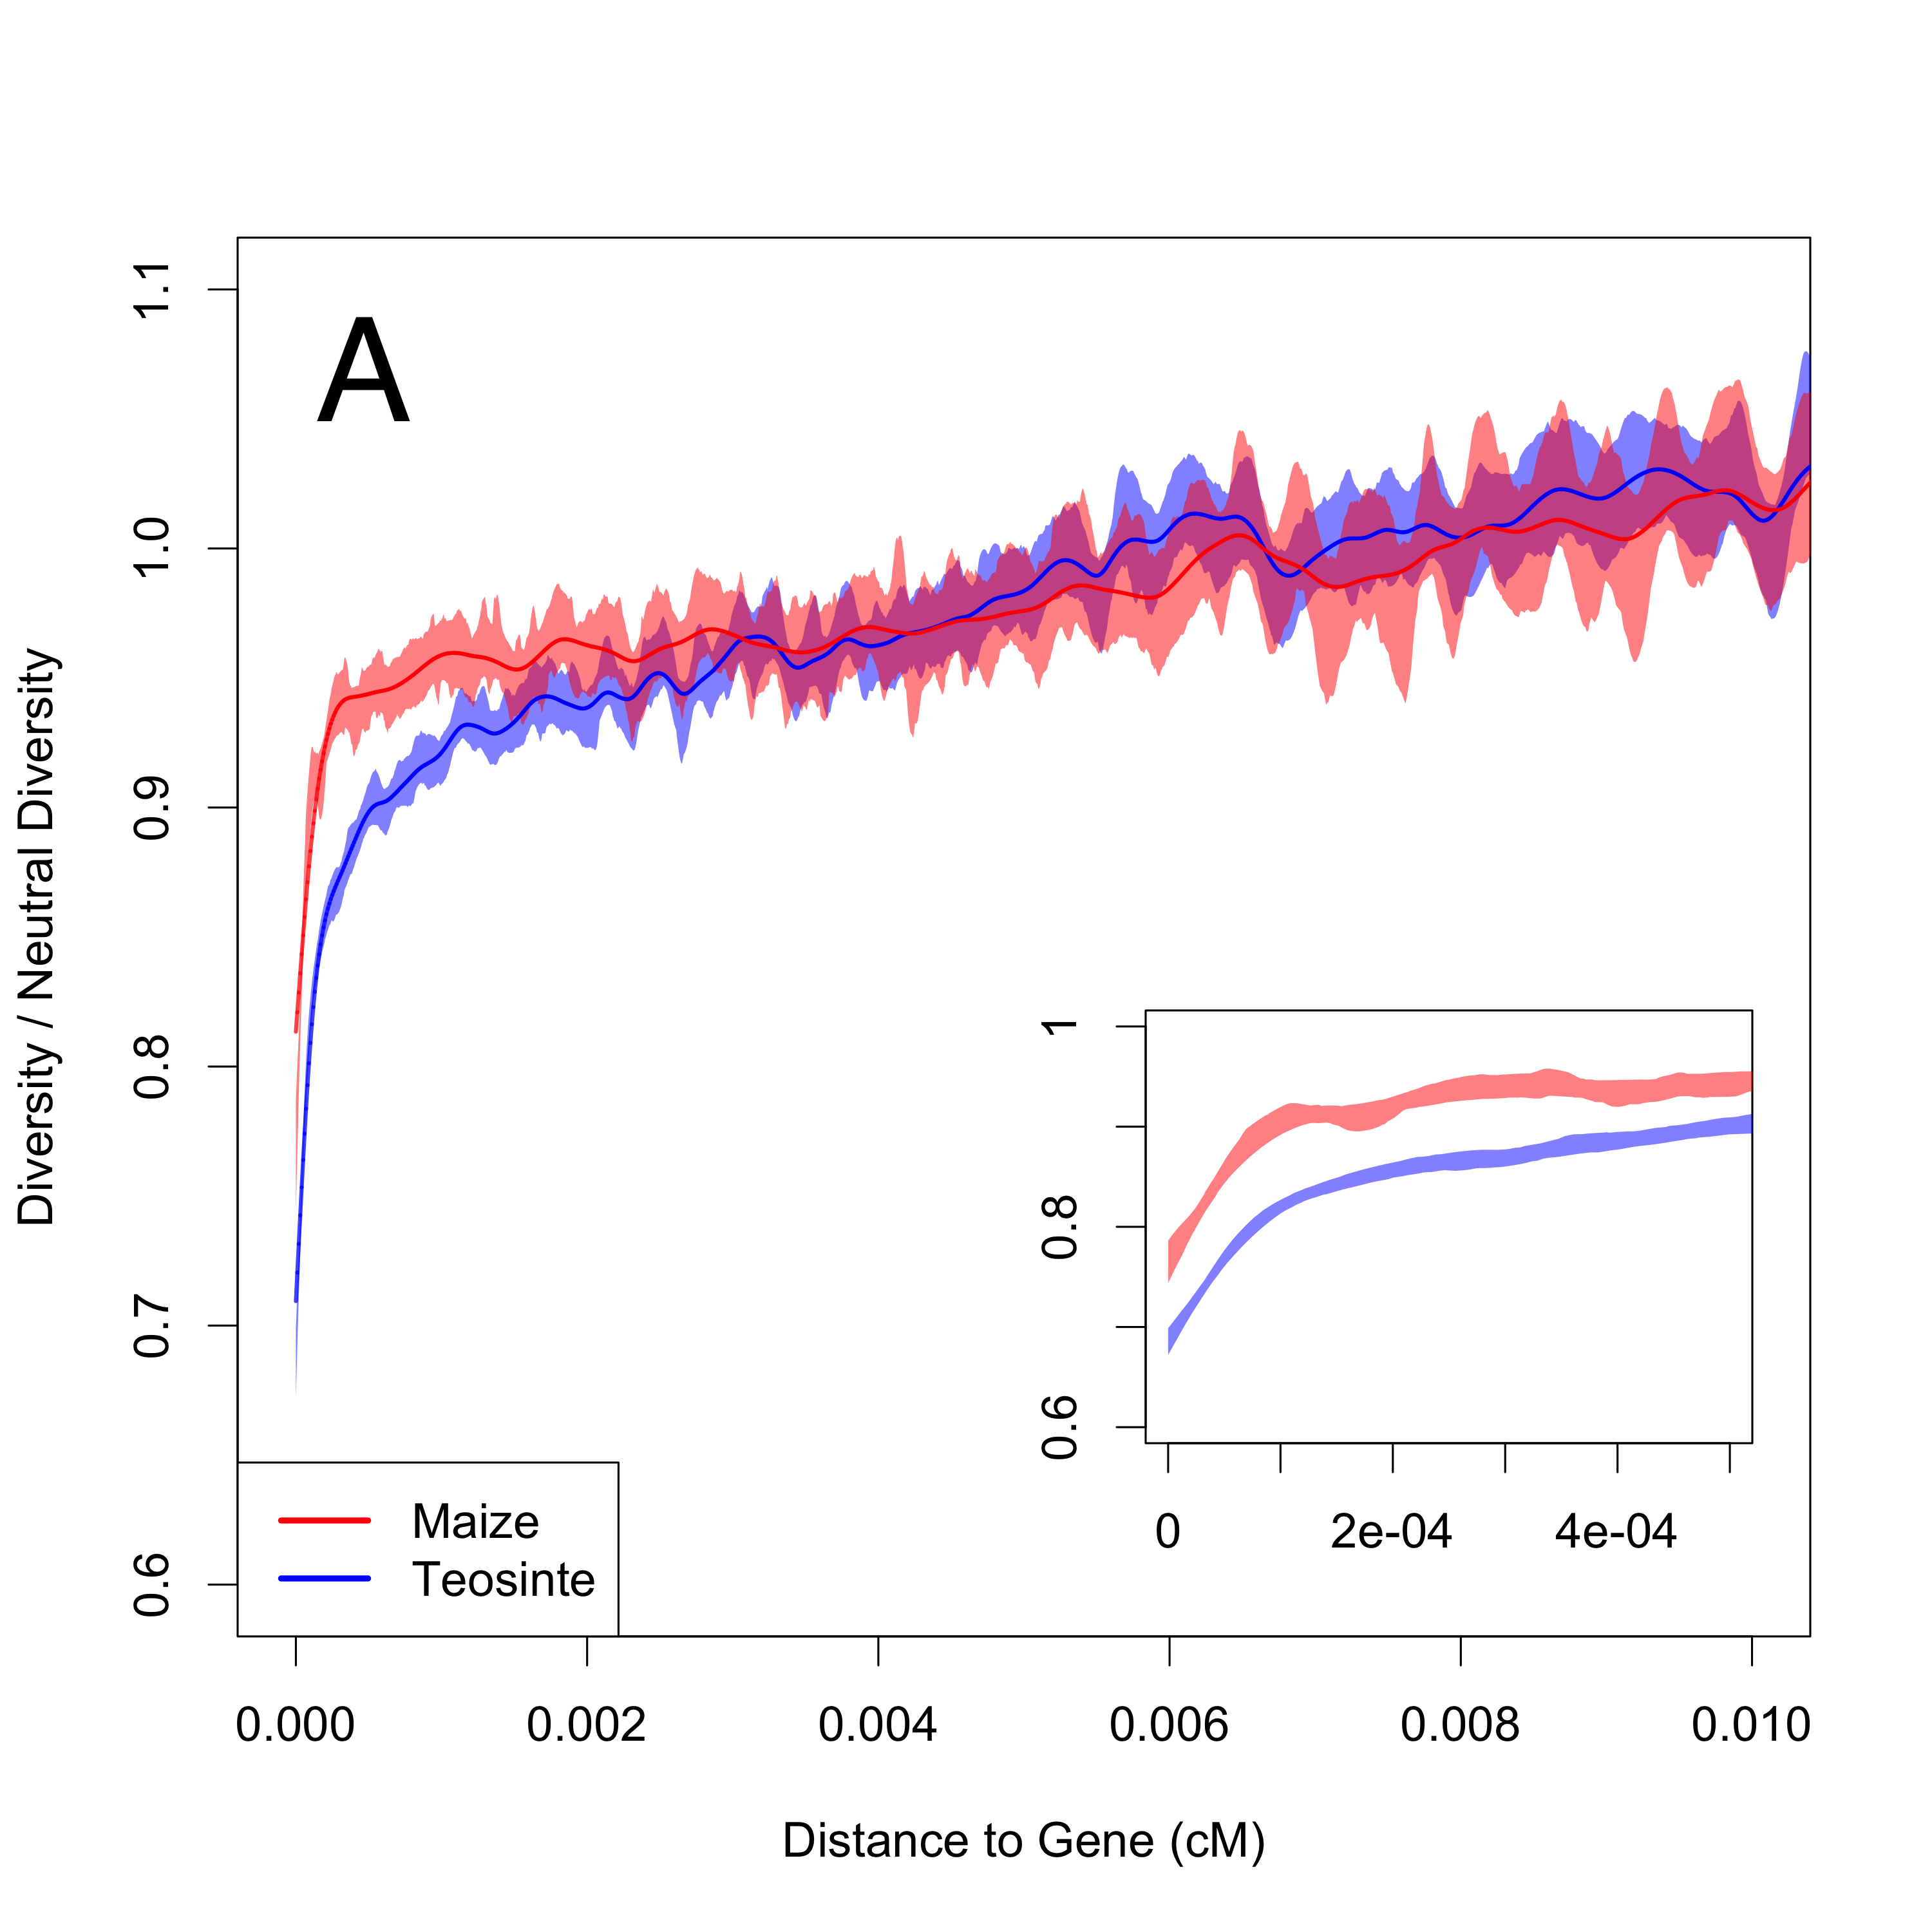
\includegraphics[width=.45\textwidth]{FigsAndFiles/distanceToGene_WithSignificance_Folded2_manuscript.png} 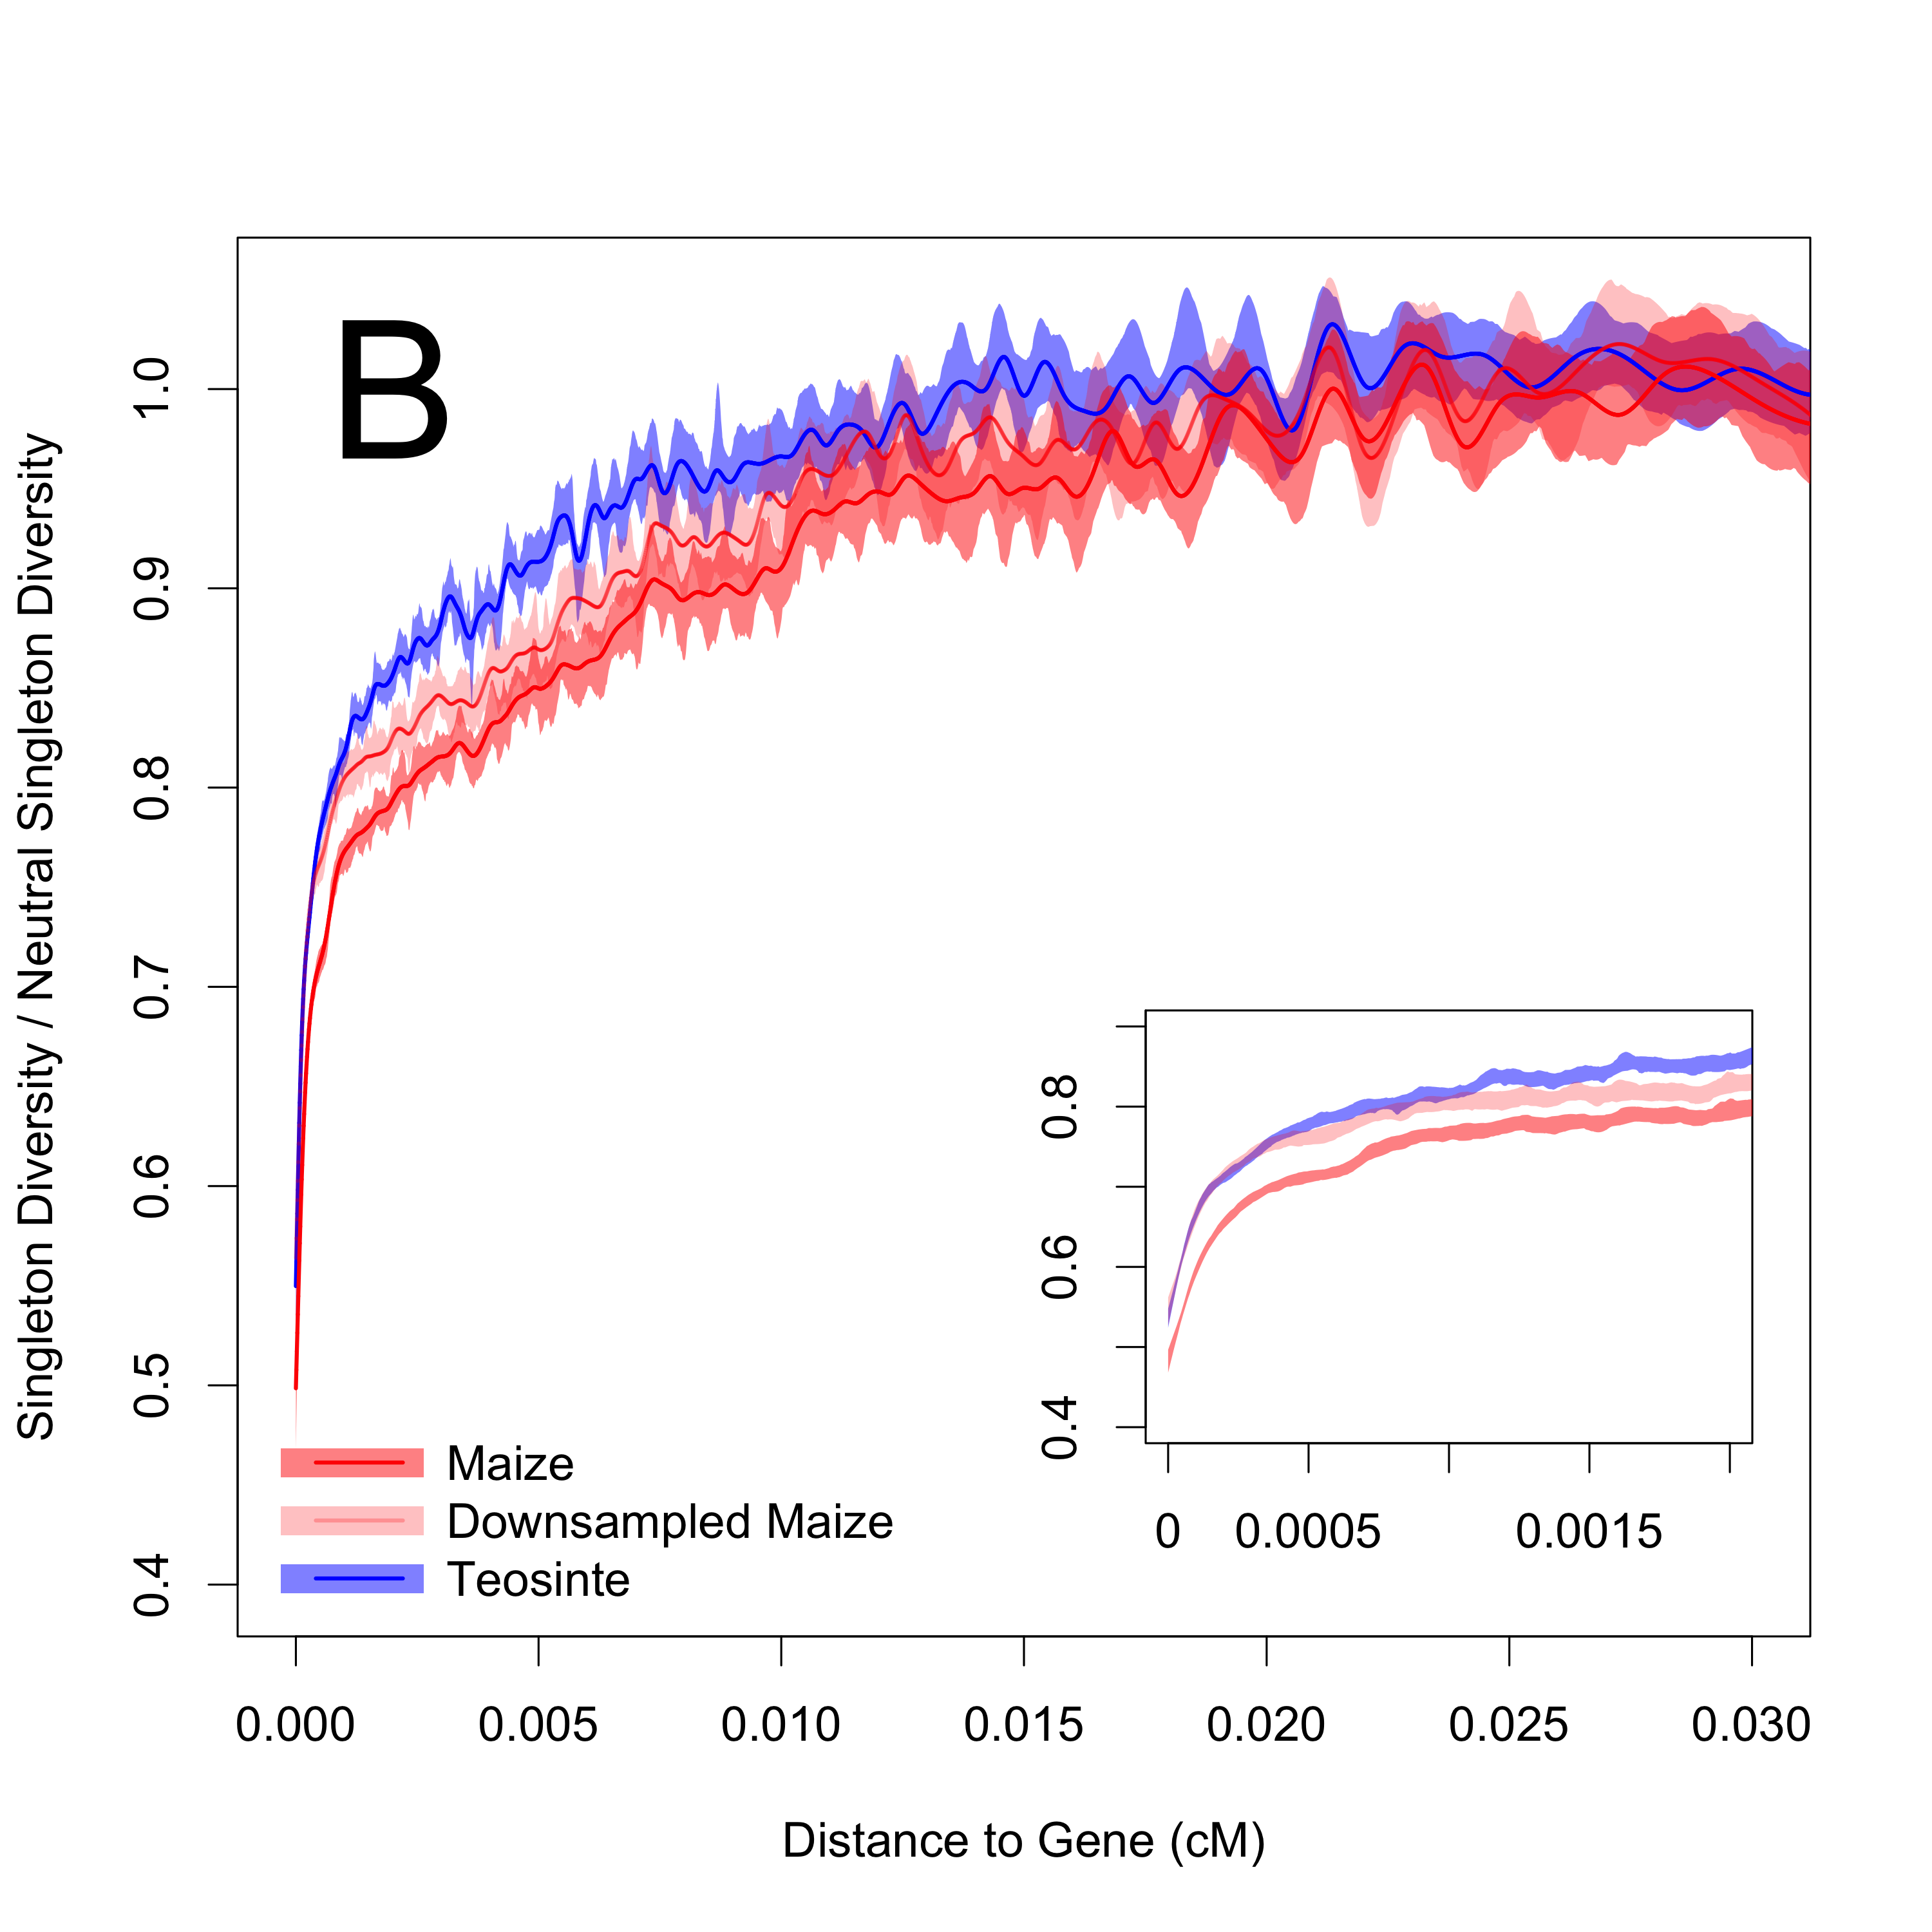
\includegraphics[width=.45\textwidth]{FigsAndFiles/distanceToGene_WithSignificance_Singletons_Downsampled_threeLines_manuscript.png}
\caption{Relative level of diversity versus distance to the nearest
  gene, in maize and teosinte. Two measures of diversity were
  investigated. \textbf{A} displays pairwise
  diversity, which is most influenced by intermediate frequency
  alleles and therefore depicts more ancient evolutionary patterns,
  and \textbf{B} depicts singleton diversity, influenced by rare
  alleles and thus depicting evolutionary patterns in the recent past. \jri{are these done with latest values we used for curve fitting? should also add the singleton vs pi comparison within species as a supplemental figure}}
\label{purify}
\end{figure*}


\textcolor{red}{This might be a good place to stick in a paragraph
  about curve fitting B to estimate s, mu.}


\subsection{Demography of maize domestication}
To explore whether differences in purifying selection between maize
and teosinte can be explained purely by demographic processes, we
first estimated the parameters of maize domestication using large-scale
sequencing data involving 23 inbred maize
landraces and 13 teosinte inbred lines included in the HapMap 2 panel
\cite{chia2012} \textcolor{red}{(supplemental table here)}. The maize
lines were collected from across the Americas and the teosinte lines
came from central Mexico. Before estimating demography, we compared
the site frequency spectrum (SFS) in genic and non-genic regions, and
observed substantial differences in the evolution of these classes of
sites. For both maize and teosinte, the SFS within genes showed a
dearth of low-frequency alleles and Tajima's D
\textcolor{red}{(reference here)} was therefore shifted
to more positive values \textcolor{red}{(figure here)}. This is consistent with the aforementioned purifying
selection and indicates that genic regions are not evolving
neutrally. Therefore, for demographic modeling we restricted analysis
to non-genic sites.

We used diffusion approximation as implemented in
dadi \cite{gutenkunst2009} to find the domestication parameters that best explain
the joint site frequency spectrum of maize and teosinte.  The model we optimized began with an
equilibrium ancestral population of size $N_a$
splitting into separate maize and teosinte populations $T_B$ generations in the past. Moving forward in
time from the split, teosinte maintained the ancestral population size, while
maize experienced an immediate effective population size change to
$N_b$ individuals, followed by exponential growth to size
$N_m$. Additionally, since the split a $M_{tm}$ individuals migrated
from teosinte into maize and $M_{mt}$ individuals migrated from maize
to teosinte.

The most likely model suggested an ancestral for $\theta$ ($4N\mu$) of
0.014734, which is similar to previous estimates
\textcolor{red}{(references here)}. Assuming a mutation rate of $\mu =
3 \times 10^{-8}$ \textcolor{red}{(reference here)}, this suggests an effective
population size of $N_a = 122,783$ individuals, a population split
$T_B = 15,523$ generations in the past, a maize bottleneck
effective populations size of $N_b = 6,455$ individuals (5.26\% of
$N_a$), a modern maize effective population size of $N_m = 366,973$
individuals, $M_{tm} = 1.35$ migrants per generation from teosinte to
maize, and $M_{mt} = 1.72$ migrants per generation from maize to
teosinte (Figure \ref{bottleneck}). We note that a population
split over 15 thousand generations before present precedes estimates
from
archaeological data which suggests maize domestication began
approximately 9,000 years before present \textcolor{red}{(reference
  here)}. This could result from multiple generations per year, or in
may reflect teosinte population structure that was present before
domestication. Also, note that the genetic time of the population
split must precede morphological changes that could be identified
morphologically.   Additionally, because recent expansion is
most evidenced by rare alleles, and since these data provide low
power to detect rare alleles, we expect that the estimate of  $N_m =
366,973$, or $\sim 3N_a$, is likely an underestimate.

We utilized a complementary dataset of 4,808 maize landrace samples collected
from across the Americas \textcolor{red}{(SeeDs reference here)} to
obtain a less downward-biased estimate of the current maize effective
population size. According to a singleton-based estimate of $\theta$
\cite{fu1993}, which was chosen since rapid post-bottleneck expansion
implies that rare alleles will most accurately reflect current maize
demography, we obtained the estimate \textcolor{red}{$N_e =
  1,011,686$}. Although less biased than the previously mentioned
esitmate, we note that ascertainment bias of the
genotyping platform used to generate these data again biases this
estimate downward.


\begin{figure}[b]
%\vspace*{.05in}
\centering
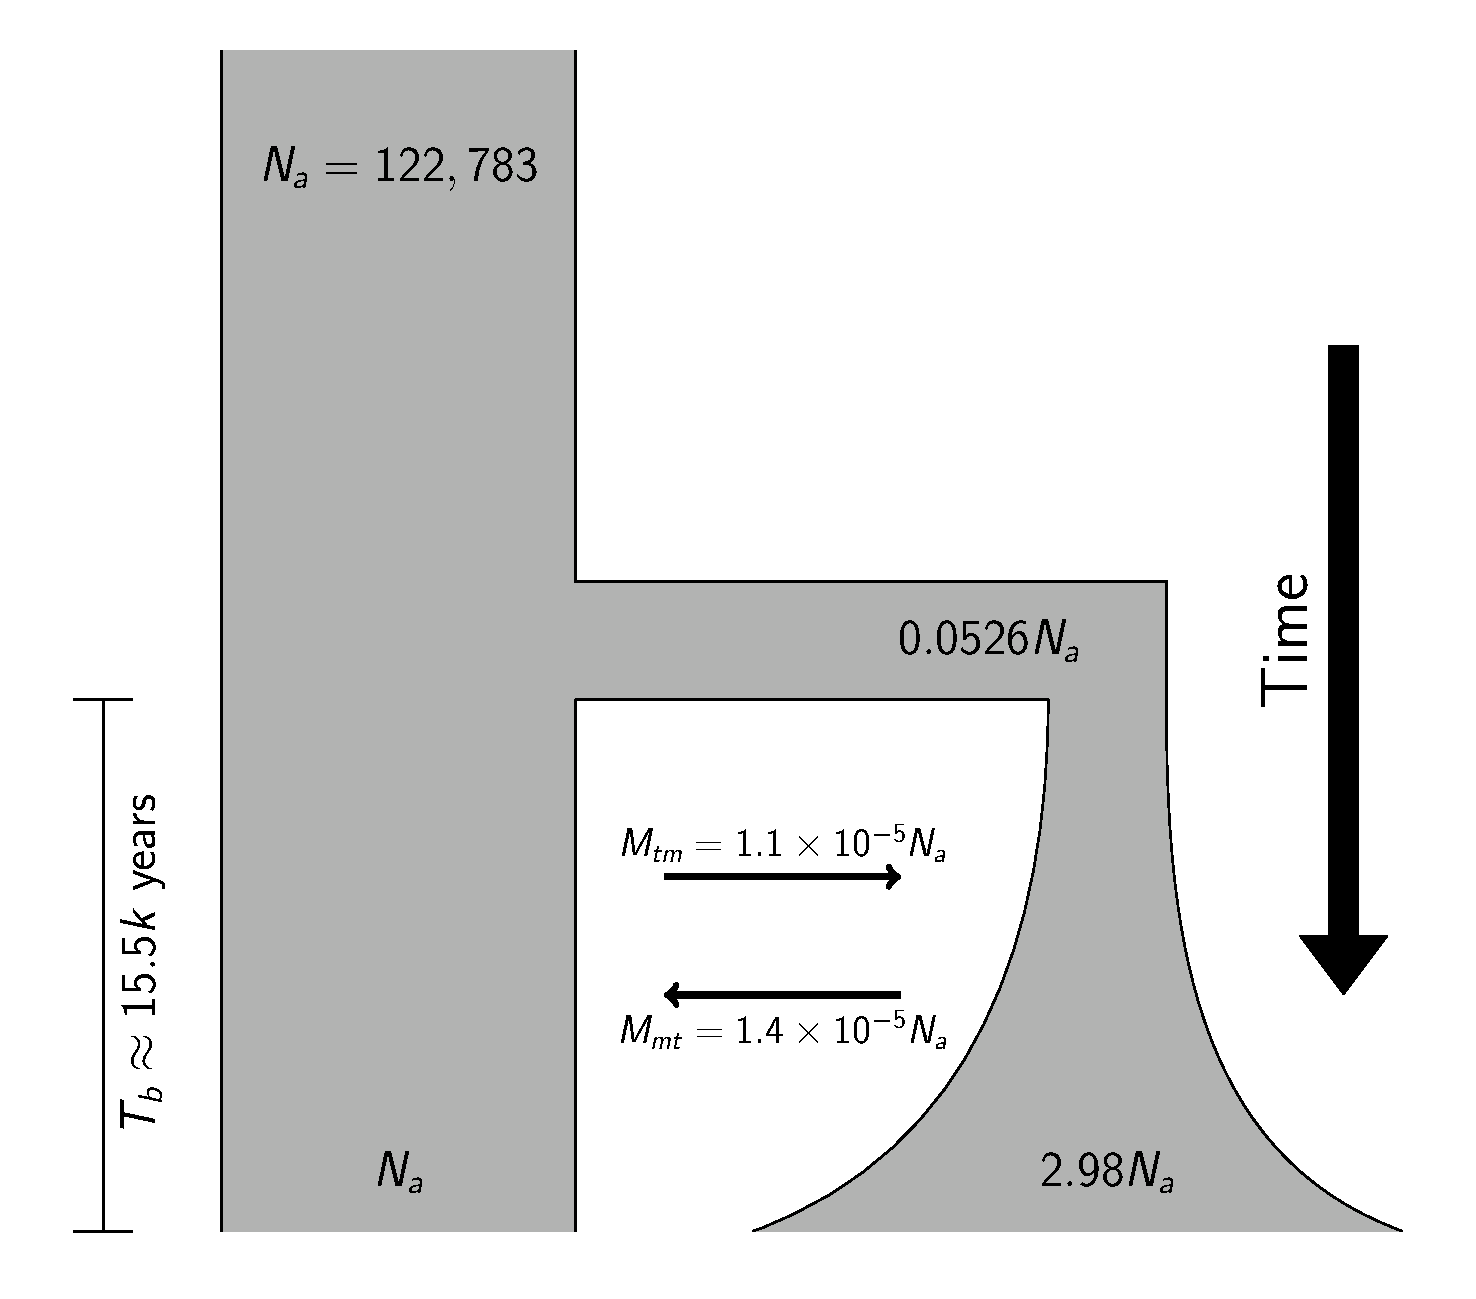
\includegraphics[width=.4\textwidth]{FigsAndFiles/DomesticationModel/domesticationModel.pdf}
\caption{Parameters of domestication as estimated by dadi. Notably,
  the maize effective population size ($N_e$) during the domestication
  bottleneck appears to have consisted of approximately 5.26\%
  the ancestral $N_e$, before recovering two at least 2.98
  times as large as the ancestral $N_e$.}
\label{bottleneck}
\end{figure}


\subsection{Simulations confirm the relationship between demographic
  processes and background selection}
\textcolor{red}{We explored whether or not the demographic patterns
  that correspond to maize domestication are capable of generating the
  interesting pattern of background selection that is observed. That
  is, does demography alone explain the weak effect of background
  selection on pairwise diversity in maize? We begain by estimating
  the distribution of fitness effects and mutation rate in both maize and teosinte from
  (formulas)... These were observed to be ZZZZZZ. Then, we simulated
  mating according to our estimated demographic model and evaluated
  the resulting levels of pairwise and singleton diversity. A LOT MORE
GOES HERE, BUT WHAT IS WRITTEN NOW CAN FRAME THINGS.}


\section{Discussion}
\subsection{Discussion 1}
Text goes here

\subsection{Discussion 2}
Text goes here

\begin{materials}
\subsection{Plant materials}
Accessions studied were selected from the Maize HapMap2
panel \cite{chia2012} . Principal component analysis was employed to ensure that
closely related individuals were not included due to their potential
to bias results \textcolor{red}{(maybe a supplemental figure here)}. Ultimately, 23 maize inbreds derived from a diverse
assortment of landraces were selected for inclusion. Thirteen teosinte
inbred lines, all members of the subspecies Z. \emph{mays}
ssp. \emph{parviglumis}, were utilized. Sequences were mapped to the
maize B73 version 3 reference genome \cite{schnable2009}
(ftp://ftp.ensemblgenomes.org/pub/plants/release-22/fasta/zea\_mays/dna/).

\subsection{Interpolating genetic position}
For many of the following analyses, physical position along a
chromosome was a less relevant measure of map location than was genetic
position. Therefore, physical positions were converted to genetic
positions by interpolating from the NAM genetic map (REFERENCE), which
provides a 1 cM resolution for physical to genetic conversion. Within
R \cite{R2014}, physical positions with corresponding genetic positions in
the NAM map were used as anchors. Physical positions in our dataset
wihout corresponding genetic position were assigned genetic positions by scaling
the anchored genetic positions according to the physical distance
between the unlabeled position and the flanking anchors.

\subsection{Estimating the site frequency spectrum}
To estimate individual  and joint site frequency spectra (SFS) for
maize and teosinte from inbred lines, each inbred individual was treated as representing
a single haplotype from its population. These were
separately computed for genic and intergenic regions, as well as for
the whole genome together. First, genic and intergenic regions were isolated using
the biomaRt package \cite{durinck2009,durinck2005} of R \cite{R2014}. Genic
regions were defined as DNA between the start and stop position of a
gene, while intergenic regions were required to be at least 5kb up- or
down-stream from a gene start/stop. With regions defined, SFS were
estimated with ANGSD \cite{korneliussen2014}. Individual population SFS were
estimated using all positions observed in at least 80\% of the
individuals in the population, and joint SFS were estimated using all
positions observed in at least 80\% of individuals in both
populations. Individuals were
assumed to be fully inbred (-doSaf 2), and subsequently allele frequencies were
divided by two to indicate haplotype frequencies. Quality filters were
employed such that reads with quality score below 30 and bases with
quality score below 20 were discarded (-minMapq 30 and -minQ 20), as were reads that didn't map
uniquely (-uniqueOnly 0). Quality scores around indels were adjusted
as in Samtools (-baq 0). Genotype likelihoods were estimated using the samtools
method (-GL 1). Major and minor alleles were inferred from the data
(-doMaf 1). Because ANGSD cannot calculate a folded joint SFS, the
maize reference genome was used for polarization and then unfolded spectra
were folded using dadi \cite{gutenkunst2009}.

\subsection{Demographic inference}

\subsection{Evaluating diversity around substitutions}
To investigate diversity around substitutions, maize and teosinte pairwise diversity was first
calculated in 1,000 kb non-overlapping windows using ANGSD
\cite{korneliussen2014}. This was performed separately for both maize and
teosinte, using the same filters as employed for estimating the
SFS. Next, SNPs and genotypes among maize, teosinte, and \emph{Tripsacum} were called. \emph{Tripsacum} bam files
were downloaded from \url{}(TRIPSICUM FILES), and then all SNPs with a
p-value less than 1e-6 were called using ANGSD. Quality filters were
as the same as before, and genotypes were only called when the
posterior probability was above 0.95. From the set of called SNPs and
genotypes, substitutions between maize and tripsicum, as well as
between teosinte and \emph{Tripsacum} were identified using R \cite{R2014} as all positions with
no more than 20\% missing data for which every maize or teosinte
allele differed from the observed \emph{Tripsacum} allele. At each class of
substitution, effects were estimated using the ensembl variant effects
predictor \cite{mclaren2010}.

For each diversity window with at least 100 bps observed, the distance from the window center to the
nearest synonymous and nonsynonymous (missense) substitution was
computed. Then, following the methods of \cite{hernandez2011}, a loess
curve was plotted for diversity values against the distance to the
nearest synonymous or nonsynonymous substitution. A span of 0.01 was
utilized. Unlike
\cite{sattath2011}, we did not fit separate loess curves in the up- and
down-stream directions, but instead fit single curves encompassing
both directions.

\subsection{Evaluating diversity around genes}
Two types of diversity surrounding genes were investigated. The first
was pairwise diversity in 1kb windows, as described previously. The
second was singleton diversity in 1kb windows. Singletons represent
the rarest class of alleles that this dataset can identify, and
collectively demonstrate the most recent patterns of evolution. Minor
allele frequencies were estimated with ANGSD \cite{korneliussen2014} using the
same quality filters previously described. Then, the number of
singletons in each non-overlapping 1kb window was calculated with R
for both maize and teosinte \cite{R2014}. For maize, we also generated a parallel set of downsampled
singleton data, for which binomial sampling within R was conducted
based on allele frequencies at each site, to generate a singleton
psuedo dataset of sample size 13, equivalent to our sample size for
teosinte. BiomaRt \cite{durinck2009, durinck2005} was then used to identify
the center of each gene. Next, the distance from each diversity window center
to the nearest gene center was computed.

Teosinte diversity is
generally higher then maize diversity. Therefore, to enable comparisons between
the reduction of diversity around genes in maize and teosinte, a
neutral measure of pairwise and singleton diversity for each taxa was
estimated. For pairwise diversity, this nuetral measure was defined according to
mean pairwise diversity at windows greater than 0.01 cM from the nearest
gene. For singletons, both maize and teosinte still showed reduced
diversity at a distance of 1 cM, so neutral diversity in this case was
defined as mean singleton diversity at positions 0.02 cM or greater
from genes. Then, pairwise and singleton diversity at each window was
standardized by dividing by the corresponding neutral
measure. Separately for pairwise and singleton diversity in maize and
teosinte, cubic smoothing splines were fit to
describe diversity levels according to the distance to the nearest
gene. Significant differences were assessed by taking 100 bootstrap
samples from each set of diversity windows and re-fitting the cubic smoothing spline to each. Then, the
2.5\% and 97.5\% quantiles of values along the bootstrapped splines
were identified.

%JRI IDEAS:
% look at SFS of SNPs by GERP score in maize vs teosinte. shift to lower freq. should be seen at lower GERP scores in maize
% discuss our estimates of deleterious mutation rate from B stuff.  these suggest only ~25% of mutations are deleterious, which contrasts results from a standard DFE
% do a standard DFE! this gives us the proportion of mutations in categories of Ns. Can use Eyre-Walker software.
% i think we do need to say something about load. add up GERP scores like Li?


\subsection{Simulations}

\end{materials}

\begin{acknowledgments}
Various thankyous will be in order. \jri{Coop and his lab. funding from NSF Biology of Rare alleles -- need grant number.}
\end{acknowledgments}


% \begin{thebibliography}{10}
% \bibitem{dadi}
% R.~Gutenkunst, R.~Hernandez,S.~Williamson, and C.~Bustamante, {\em
%   Inferring the joint demographic history of multiple populations from
%   multidimensional SNP frequency data}, PLoS Genetics., 5:10 (2009), e1000695.

% \bibitem{hapmap2}
% J.~Chia, C.~Song, P.~Bradbury, D.~Costich, N.~de~Leon, and others,
% \emph{Maize HapMap2 identifies extant variation from a genome in
%   flux}, Nature Genetics., 44 (2012), 803-807.

% \bibitem{maizeGenome}
% P.~Schnable, D.~Ware, R.~Fulton, J.~Stein, F.~Wei, \emph{The B73 maize
% genome:complexity, diversity, and dynamics}, Science., 326:5956
% (2009), 1112-1115.

% \bibitem{angsd}
% T.~Korneliussen, A.~Albrechtsen, and R.~Nielsen, \emph{ANGSD: Analysis of
% next generation sequencing data}, BMC Bioinformatics., 15:356 (2014),
% 10.1186/s12859-014-0356-4.

% \bibitem{R}
% R Core Team, \emph{R: A language and environment for statistical
%   computing}, R Foundation for Statistical Computing., Vienna,
% Austria.

% \bibitem{biomaRt1}
% S.~Durinck, P.T.~Soekknabm E.~Birney, and W.~Huber, \emph{Mapping
%   identifiers for the integration of genomic datasets with the
%   R/Bioconductor package biomaRt}, Nature Protocols., 4 (2009),
% 1184-1191.

% \bibitem{biomaRt2}
% S.~Durinck, Y.~Moreau, A.~Kasprzyk, S.~Davis, B.~De~Moor, and others,
% \emph{BioMart and Bioconductor: a powerful link between biological
%   databases and microarray data analysis}, Bioinformatics, 21 (2005),
% 3439-3440.

% \bibitem{vep}
% W.~McLaren, B.~Pritchard, D.~Rios, Y.~Chen, P.~Flicek, and
% F.~Cunningham, \emph{Deriving the consequences of genomic variants
%   with the Ensembl API and SNP Effect Predictor}, Bioinformatics,
% 26:16 (2010), 2069-2070.

% \bibitem{hernandez11}
% R.D.~Hernandez, J.L.~Kelley, E.~Elyashiv, S.C.~Melton, A.~Auton, and
% others, \emph{Classic selective sweeps were rare in recent human
%   evolution}, Science, 331:6019 (2011), 920-924.

% \bibitem{sattath11}
% S.~Sattath, E.~Elyashiv, O.~Kolodny, Y.~Rinott, and G.~Sella,
% \emph{Pervasive adaptative protein evolution apparent in diversity
%   patterns around amino acid substitutions in Drosophila simulans},
% PLoS Genetics, 7:2 (2011), e1001302.

% \bibitem{charlesworth93}
% B.~Charlesworth, M.~T.~Morgan, and D.~Charlesworth, \emph{The Effect
%   of Deleterious Mutations on Neutral Molecular Variation}, Genetics,
% 134 (1993), 1289-1303.

% \end{thebibliography}

\bibliography{Reference}
\bibliographystyle{pnas}
%\nocite{*}


\end{article}
\end{document}